\documentclass{chi2009}
\usepackage{times}
\usepackage{url}
\usepackage{graphics}
\usepackage{color}
\usepackage{wrapfig}
% \usepackage{picins}
% \usepackage{floatflt}
\usepackage[pdftex]{hyperref}
\hypersetup{%
pdftitle={Mashing the Ideas Expressed on the Web},
pdfauthor={Beth Trushkowsky and Rob Ennals},
pdfkeywords={CSCW, sensemaking, web, browsers, collaboration, mind mapping},
bookmarksnumbered,
pdfstartview={FitH},
colorlinks,
citecolor=black,
filecolor=black,
linkcolor=black,
urlcolor=black,
breaklinks=true,
}

\newcommand{\todo}[1]{}
% \newcommand{\todo}[1]{\footnote{{\bf TODO:} #1}}
\newcommand{\Intel}{Intel\textsuperscript{\textregistered}}

\newcommand{\idea}[1]{{\color{blue} IDEA: #1}\\}
\newcommand{\studyresult}[1]{{\color{red} STUDY RESULT?: #1}\\}
\newcommand{\howmany}{{\color{red} (HOW MANY?)}}

\pagenumbering{arabic}  % Arabic page numbers for submission.  Remove this line to eliminate page numbers for the camera ready copy


\begin{document}
% to make various LaTeX processors do the right thing with page size
\special{papersize=8.5in,11in}
\setlength{\paperheight}{11in}
\setlength{\paperwidth}{8.5in}
\setlength{\pdfpageheight}{\paperheight}
\setlength{\pdfpagewidth}{\paperwidth}
%
\toappear{Submitted to the Tinkering, Tailoring, and Mashing workshop at CSCW 2008}

\title{Participatory Mashups: Using Users to make Data Mashable}

\numberofauthors{2}

%\author{
%	\alignauthor Authors anonymized for submission
%}

\author{
\alignauthor Rob Ennals\\
       \affaddr{Intel Research}\\
       \affaddr{2150 Shattuck Avenue}\\
       \affaddr{Penthouse Suite}\\
       \affaddr{Berkeley, CA 94704, USA}\\
       \email{robert.ennals@intel.com}
\alignauthor Beth Trushkowsky\\
       \affaddr{Computer Science Division}\\
       \affaddr{University of California at Berkeley}\\
       \email{trush@berkeley.edu}
}
\sloppy 

\maketitle

\begin{abstract}
Most mashups concern themselves with data that is fairly easy for a machine to understand: addresses, phone numbers, information available through APIs, or information that can be scraped from a small set of popular web sites.

However much of the most interesting information on the web is not in a form that a computer can easily understand. It may be in natural language text, or it may be in the long tail of web sites that developers have not found it worthwhile to write scrapers for.

In this paper, we promote the approach of ``participatory mashups'' in which the users of the mashup also teach the mashup ways that it can understand new data. As examples, we present our work on Think Link, which connects factual statements on the web to related statements elsewhere, and Mash Maker, which attempts to understand the meaning of structured data on arbitrary web pages.
\end{abstract}


\section{Introduction}

If we understand what the information on a page means then we can do useful things with it. We can connect the information to information elsewhere that might be relevant, we can compute new information from the information we have, and we can present users with new interfaces that are more useful than that provided by any individual site. 

Some kinds of information are easier to understand than others, and mashups have so far understandably focussed on the low-hanging fruit. Addresses follow an easily recognized pattern, and have led to a large number of useful mashups which plot various things on maps or work out what things are near to other things. Similarly, many mashups have made use of data that is available from APIs, or that can be easily scraped from popular web pages that the mashup has been hard-coded to understand.

But what about everything else? 

Much of the most interesting information on the web is available as unstructured natural language text: arguments, ideas, opinions, factual claims, jokes. Much of this is information that could benefit a lot from being mashed up. For example ``which of these claims is likely to be wrong?'', ``what other sites disagree with this opinion?'', ``is there a more reliable source that backs up this claim?'', or ``what ideas on this site would I be likely to find most interesting?''.

Similarly, there is a lot of structured information stored in the ``long tail'' of web sites that are too small for it to be worth a mashup author writing a custom scraper or API interface for, but which may nonetheless be very interesting. For example, tables of data that have been entered by hand, or one of the many tiny web services that display data from a database backend using their own custom template that nobody has ever written a scraper for.

In this approach we argue for ``participatory mashups'' as a way to open up access to this data. In a participatory mashup we blur the line between the users and creators of a mashup by allowing the users of a mashup to teach the mashup how to understand new information, and connecting information in new ways. By teaching a participatory mashup the meaning of some data, the user helps themselves, since they can now include this data in their mashup, but they also help the wider community of users, since all other users can now benefit from the system understanding this data.

We motivate this approach using two mashup tools that we have built. Think Link allows users to identify factual claims that they read on web pages and connect them to related factual claims on other sites, including claims that may oppose the original claim. Mash Maker allows users to teach it the meaning of structured data on arbitrary web sites, and then enhances these web sites to make them more useful, guided by example improvements provided by users.

More generally, we consider a tool to be a ``participatory mashup'' if it relies on users to teach it what information on the web means, and how that information is connected together. We argue that this is an approach that other applications could also use to help them understand the web.

\section{Think Link}

\begin{figure}[tb]
	\begin{center}
	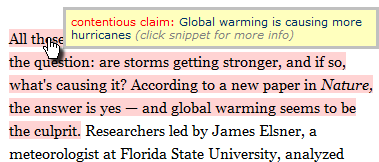
\includegraphics[width=6cm]{../screenshots/highlight_crop.png}
	\caption{Hovering over a highlighted snippet shows a summary}
	\label{highlight}
	\end{center}
\end{figure}

\begin{figure}[tb]
	\begin{center}
	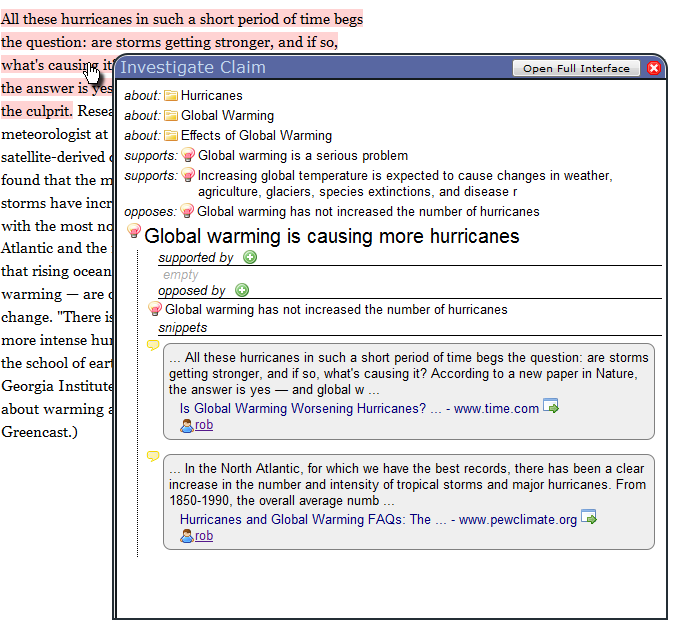
\includegraphics[width=6cm]{../screenshots/claim_popup_crop2.png}
	\caption{Click on a claim to investigate evidence for and against it}
	\label{claimview}
	\end{center}
\end{figure}

\begin{figure}[tb]
	\begin{center}
	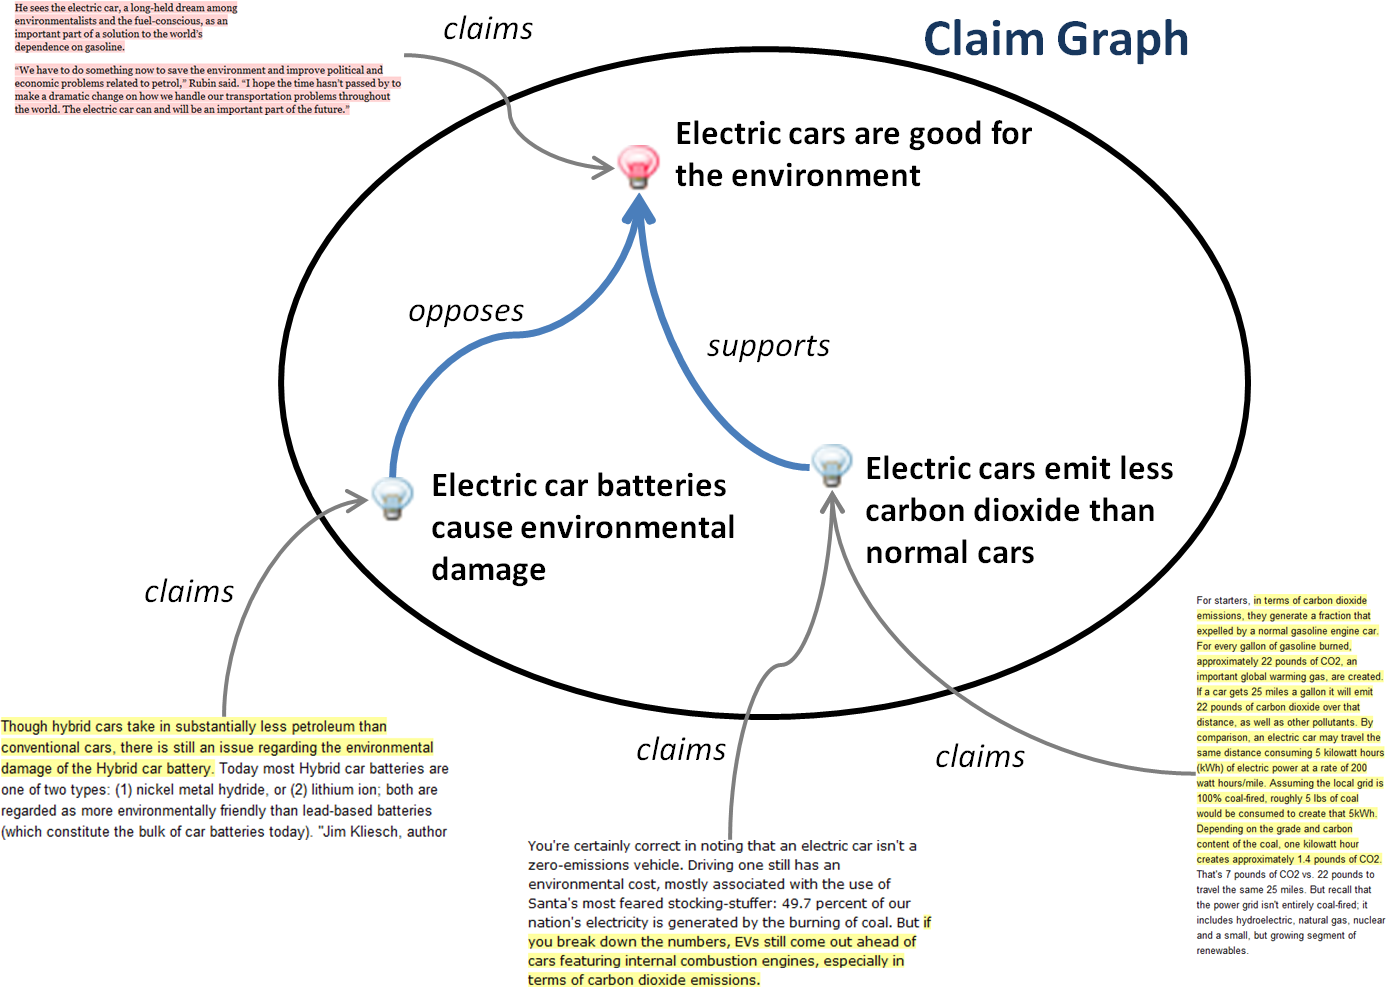
\includegraphics[width=7.7cm]{../screenshots/summary_graph.png}
	\caption{Think link connects claims to each other and to web snippets}
	\label{summarygraph}
	\end{center}
\end{figure}

\begin{figure}[tb]
	\begin{center}
	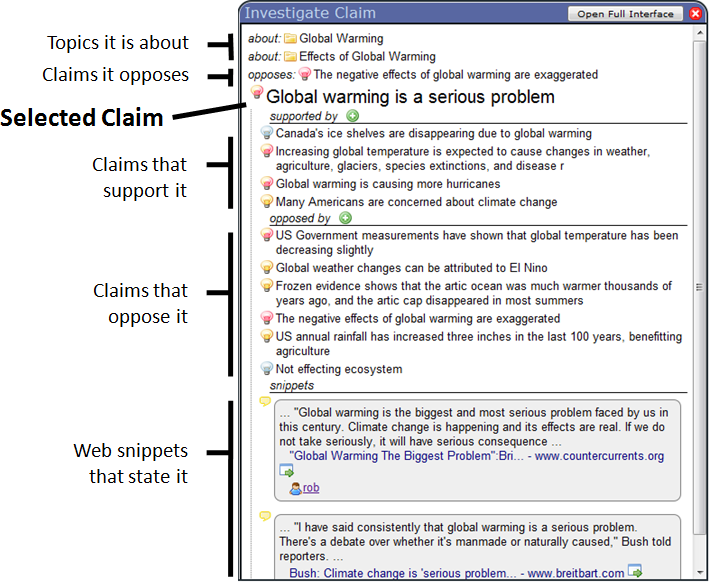
\includegraphics[width=8cm]{../screenshots/claimbrowse_diagram.png}
	\caption{The claim browser visualizes the claim graph}
	\label{claimbrowse_diagram}
	\end{center}
\end{figure}


Much concern has been expressed recently about biased or inaccurate information on web sites~\cite{bbcwebwarning,wikifalse}, and the media echo chamber problem in which people read web sites that feed their own views back to them, rather than exposing them to the opposing opinions held by other groups~\cite{echochamber,echochamber2}. 

Think Link~\cite{thinklink} is a Firefox extension that helps users evaluate the truth of statements they read, helps users be more easily exposed to a range of ideas and opinions that they might not otherwise encounter.

As a user browses the web, Think Link highlights snippets of text that other users have identified as making claims that are interesting or contraversial (Figure~\ref{highlight}). Interesting claims are highlighted in yellow, and contraversial claims are highlighted in red. If a user clicks on a highlighted snippet, Think Link will display an interface that allows a user to easily find snippets on other web pages that make related claims, including snippets that argue against the opinion put forward by the highlighted snippet (Figures~\ref{claimview} and \ref{claimbrowse_diagram}). Think Link allows a user to easily access the best arguments for and against a claim, including arguments they might not otherwise have come across because they would not have been voiced by the web sites that the reader normally reads.

Think Link maintains a graph of known factual claims, their relationship to each other, and the snippets that hold these claims (Figure~\ref{summarygraph}). This graph is built entirely by users of the tool. Users create claims, users connect claims, and users identify snippets making claims. Similarly, users vote for snippets, claims, or connections that they believe are particularly important.

This graph allows one to ask interesting questions such as ``Which snippets on this page make claims that are opposed by snippets elsewhere on them web?'', ``What is the most trustworthy news source that makes this claim?'', ``What do my friends think about this idea?'', ``What are the most interesting claims about this topic that I haven't read before'', or ``What is the best argument against this claim, and what would be the best counter-argument to that?''.

\begin{figure*}[tb]
	\begin{center}
	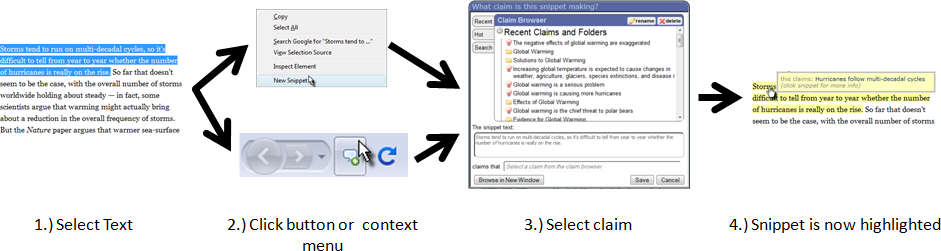
\includegraphics[width=14cm]{../screenshots/newsnip_all.png}
	\caption{Process for creating a new snippet}
	\label{createprocess}
	\end{center}
\end{figure*}

Identifying factual claims and the connections between them automatically would be very difficult using the current generation of natural language processing and automated reasoning tools; however this is quite an easy task for humans.  To create a new snippet, a user selects the text that is making an interesting factual claim, and then uses a claim browser interface to identify the claim being made (Figure~\ref{createprocess}). Users can connect claims together using a simple drag and drop interface.

Our user study participants identified several reasons why they would want to mark up factual claims in documents they found. The most common reason people gave for identifying and organizing factual claims was if the person was writing an article or researching a topic and wanted to keep track of the information they had found. One user (who is an active blogger) also expressed an interest in finding and marking up instances of claims that he disagreed with, so that readers would see the arguments highlighted in red and be directed to the counter-arguments. The same user also expressed an interest in marking up claims in documents he had made in his own articles so that readers could quickly see the evidence he had found in support of his claims. 

Like the work of Luis von Ahn~\cite{vonahn,recaptcha} or the ``invisible hand'' or Adam Smith the intention is that people should be motivated by self interest to do something that benefits the wider community.



\section{Mash Maker}

Mash Maker~\cite{mashmaker} is a browser extension that understands the meaning of the pages that users browse and suggests ways that it can improve the current page so as to be more useful to the user. Mash Maker relies on users to teach it both how to understand web pages, and also how particular kinds of web page might be improved in interesting ways.

As views a web page, Mash Maker will suggest ways that it can make the page more useful, and suggest these improvements on its toolbar. If the user clicks on the button for such an improvement then Mash Maker will apply it to the current page, potentially using other web sites and remote APIs, and potentially applying widgets that produce new visualizations or compute new data (Figure~\ref{mapinsert}). Mash Maker suggests improvements based on the meaning of the current page, the meaning of pages that the user has recently browsed, and the behaviour of other users.

Our intention is that users should be able to use Mash Maker to enhance arbitrary web sites in arbitrary ways. Unlike ``mashup creation tools'' like Yahoo Pipes~\cite{pipes} or Microsoft Popfli~\cite{popfly}, we see Mash Maker not a tool for creating special-case mashup sites, but as a generalized tool that understands what you are doing and infers new mashups that can enhance your current experience, based on what others have tried in the past. 

Users can contribute to Mash Maker in several different ways. They can teach Mash Maker how to understand new kinds of web site, they can write new widgets, and they can show Mash Maker new ways that it can improve web pages that contain particular kinds of data. A user teaches Mash Maker how to extract information from a particular kind of web page by opening the Mash Maker extractor editor (Figure~\ref{extractedit}) and picking out examples of things on the page that the user thinks is interesting. As more users give Mash Maker more examples, Mash Maker gets better at understanding what pages mean. Unlike tools like Dapper~\cite{dapper} extractors are not owned by particular users. Instead an extractor is built up from examples given by all users on the web. 

Given the huge number of differently formatted web sites on the web, it would not be practical for Mash Maker to be able to understand such a large range of web sites without users participating to teach in what different sites mean. For the users, the benefit of teaching Mash Maker how to understand a web site is that they get to use an enhanced version of the web site that Mash Maker has improved for them.


\begin{figure}[tb]
	\begin{center}
	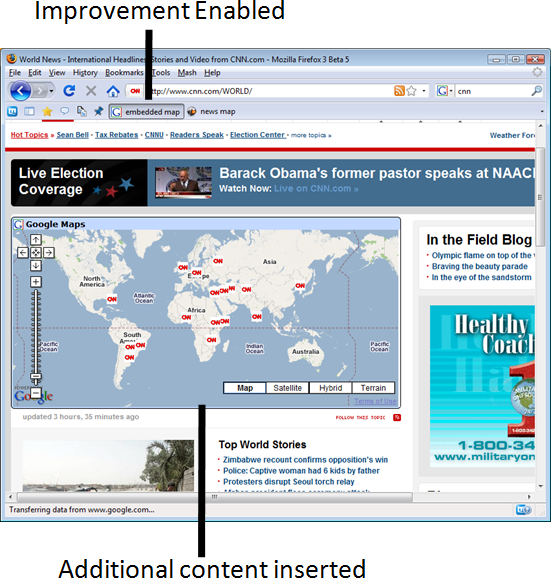
\includegraphics[width=6cm]{../mmpics/mapinsert.png}
	\caption{Using Mash Maker to add a map to a page}
	\label{mapinsert}
	\end{center}
\end{figure}

%\begin{figure}[tb]
%	\begin{center}
%	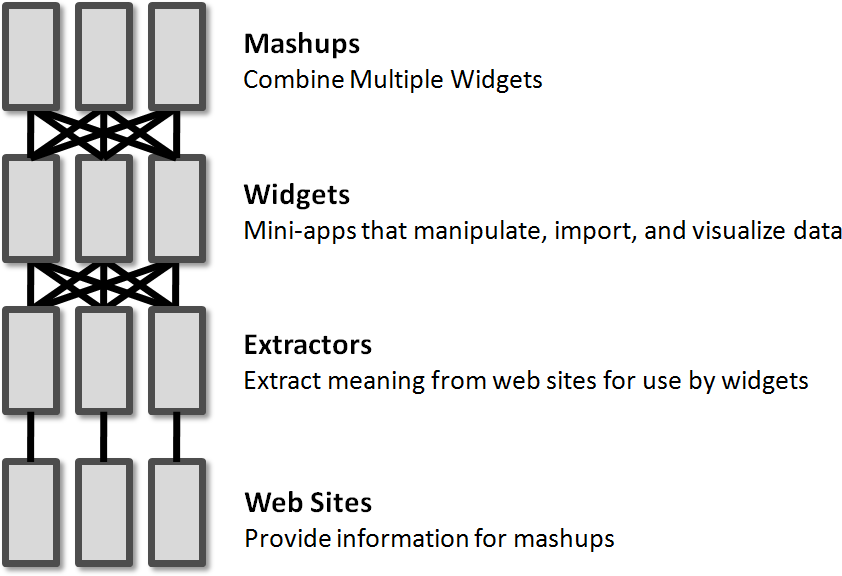
\includegraphics[width=6cm]{../mmpics/layers.png}
%	\caption{The layers of Mash Maker}
%	\label{layers}
%	\end{center}
%\end{figure}


\begin{figure}[tb]
	\begin{center}
	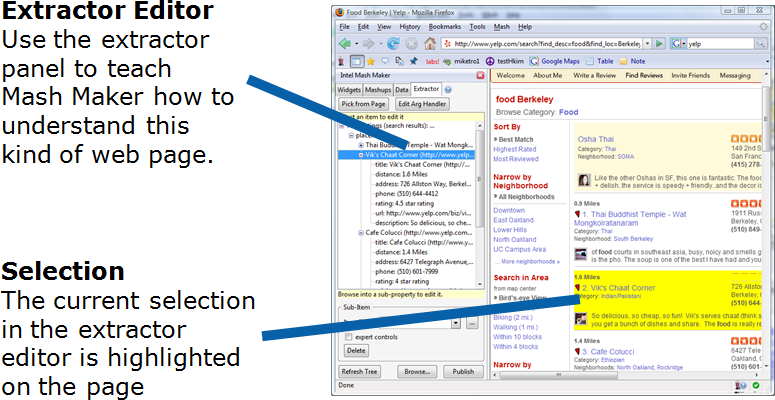
\includegraphics[width=8cm]{../mmpics/extractor_summary.png}
	\caption{Any user can teach Mash Maker how to understand new pages}
	\label{extractedit}
	\end{center}
\end{figure}


\section{Patterns vs Instances}

Users teach Mash Maker ``patterns'' that Mash Maker can use to understand a large number of similarly formatted web pages (e.g. how to understand a flight listing on expedia). This differs from Think Link, in which users pick out individual instances of factual claims which are not generalized to automatically find more snippets.

In the future, we plan to extend Think Link with natural language processing technology so that Think Link can automatically find new snippets, based on the examples it has been given. For example, if many users have shown Think Link example snippets that make the claim ``global warming is man made'', then Think Link could use these examples to find other snippets that may also be making this claim. At the simplest level, this could be done using simple textual similarity, similar to that done by Google Book Quotations~\cite{quotations}.


\section{Related Work}

The notion of a ``participatory mashup'' is somewhat fuzzy, and indeed some previous work can be considered to fit this description to some extent. To be a ``true'' participatory mashup, we believe a tool should not just allow users to contribute content, but allow users to teach it how to understand the meaning of content that already exists on the web, and use this knowledge to help other users of the tool.

reCAPTCHA~\cite{recaptcha} gives users the task of correctly transcribing scanned books as a test to see if they are human. Users thus unintentionally help machines better understand this information. Luis von Ahn has also shown how users can be persueded to teach a system what data means by making it fun~\cite{vonahn}. Our approach to persueding users to teach us what data means is to make this data immediately useful to them.

Online mashup creation tools such as Yahoo Pipes~\cite{pipes} or Microsoft Popfly~\cite{popfly} allow users to contribute new mashups. These tools treat each mashup as a separate entity and do not enable users to contribute knowledge about the web that can be used by other mashups.

Dapper~\cite{dapper} allows users to create new web scrapers, effectively creating APIs from web sites. This is similar to the extractor editor in Think Link. The key difference is that each scraper users create is treated as a separate entity, owned by a particular user, rather than as a pool of knowledge about the web that can be shared and edited by all users.

Like Think Link, SpinSpotter~\cite{spinspotter} also uses a browser plugin to help users identify and share instanes of media bias and misrepresentation. SpinSpotter allows users to annotate web pages with comments about the spin they think is present and suggest textual edits. This differs from Think Link, which attempts to understand what claims are being made and relate them to claims made elsewhere on the web.

FreeBase~\cite{freebase} is an open database of knowledge that anyone can contribute to. While FreeBase does not understand the meaning of existing web sites, it does allow users to contribute knowledge that mashups can use.



\section{Acknowledgments}

We would like to think Allison Woodruff, Tye Rattenbury, Prashant Gandhi, Eric Brewer, and all our user study participants for all their help during the design of Think Link and Mash Maker. Think Link and Mash Maker both use icons from the free FamFamFam Silk~\cite{silkicons} collection.

\bibliographystyle{abbrv}
\bibliography{biblio}

\end{document}

